\chapter{Systembeskrivelse}
Det udviklede system består af en biomedicinsk måleopstilling med en hardware- og tilhørende softwaredel. Systemet er en invasiv blodtryksmåler udviklet til forskning. Blodtryksmålesystemet skal kunne tilsluttes et måleobjekt og kontinuerligt monitorere blodtrykket. På Figur 4.1 ses illustrationen af systemets opsætning.  

\begin{figure}[H]
	\centering
	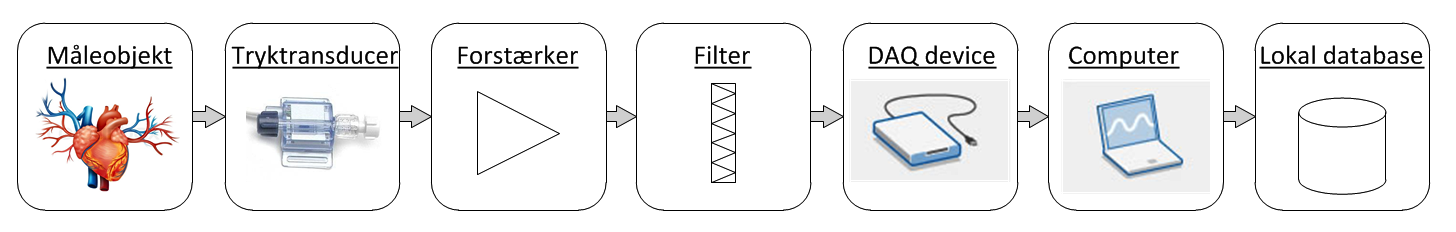
\includegraphics[width=1\textwidth]{Figurer/Snip20151209_73}
	\caption{Illustration af systemet}
\end{figure}

Den udviklede hardwaredel er opbygget som et elektrisk kredsløb bestående af en forstærker og et filter, der behandler signalet. Det tryk, der ønskes behandlet kommer fra et Måleobjekt og transformeres via en Tryktransducer. Tryktransduceren har til formål at konvertere Måleobjektets fysiske tryk til et analogt signal. Efter konverteringen fra tryk til et analogt signal forstærkes signalet i forstærkeren. Forstærkningen er nødvendig, da Tryktransducerens spændingssignal er meget svagt, og skal derfor forstærkes op til en spænding, der udnytter DAQ'ens måleområde bedst muligt. Derudover skal signalet filtreres i det indbyggede analoge filter, hvor signalet frasorterer frekvenser, der er højere end 50 Hz, da disse frekvenser er irrelavante for blodtrykssignalet. Når signalet har passeret Forstærker- og Filterblokken, konverteres det i DAQ’en fra det analoge signal til et digitalt signal, hvorefter signalet kan behandles af softwaren. \\\\
Blodtryksmålesystemets softwaredel er udviklet til at monitorere blodtrykssignalet grafisk som funktion af tiden. Softwaren er programmeret i Visual Studio C\#, og er udviklet til at være anvendelig i forskningssammenhænge. Brugergrænsefladen skal grafisk vise blodtrykssignalet kontinuert samt opdatere og udskrive de hæmodynamiske data. Systemet skal ligeledes kunne kalibreres, nulpunktsjusteres, anvende digitalt filter samt gemme målinger på en lokal database. 
